\documentclass[12pt]{article}
\usepackage{amsmath}
\usepackage{amssymb}
\usepackage{cancel}
\usepackage{graphicx}
% \usepackage{physics}
\usepackage{siunitx}
\usepackage{wrapfig}

% \AtBeginDocument{\RenewCommandCopy\qty\SI}

\newcommand{\E}[1]{\times 10^{#1}}

\title{
    Chapter 17 End-of-Chapter Problems
    \\ \small
    Halliday \& Resnick, 10th Edition
}

\author{Donald Aingworth IV}

\date{\small Hit me where it Matters}

\begin{document}
    \DeclareSIUnit{\atm}{atm}
    \DeclareSIUnit{\cal}{\ cal}
    \DeclareSIUnit{\Cal}{\ Cal}
    \DeclareSIUnit{\calorie}{\ cal}
    \DeclareSIUnit{\Calorie}{\ Cal}
    \DeclareSIUnit{\celsiusdegree}{C^\circ}
    \DeclareSIUnit{\fahrenheit}{^\circ F}
    \DeclareSIUnit{\fahrenheitdegree}{F^\circ}
    \DeclareSIUnit{\torr}{\ torr}

    \maketitle

    \begin{center}
        \textit{Where needed in the problems, use}\\
        speed of sound in air = 343 m/s\\
        \textit{and}\\
        density of air = 1.21 \unit{\kilo\gram/\meter^3}\\
        \textit{unless otherwise specified.}
    \end{center}

    \pagebreak
    \section{Problem 1}
        Two spectators at a soccer game see, and a moment later hear, the ball being kicked on the playing field. 
        The time delay for spectator A is 0.23 s, and for spectator B it is 0.12 s. 
        Sight lines from the two spectators to the player kicking the ball meet at an angle of 90\unit{\degree}. 
        How far are (a) spectator A and (b) spectator B from the player?
        (c) How far are the spectators from each other?

        \subsection{Solution (a)}
            This is a simple question to answer.
            The distance traveled to A would be equal to the speed of sound times the time taken to travel the distance.
            \begin{align}
                x   &=  vt
                    =   (343\,\unit{\meter/\second})(0.23\,\unit{\second})
                    =   \boxed{78.89\,\unit{\meter}}
            \end{align}

        \subsection{Solution (b)}
            The is calculatable the same way.
            \begin{equation}
                y   =   vt
                    =   (343\,\unit{\meter/\second})(0.12\,\unit{\second})
                    =   \boxed{41.16\,\unit{\meter}}
            \end{equation}

        \subsection{Solution (c)}
            The 90 degree angle of their sight lines makes the triange of the two spectators and the ball a right triangle, so we can use the Pythagorean theorem to find the distance between the spectators.
            \begin{equation}
                h   =   \sqrt{x^2 + y^2}
                    =   \sqrt{(78.89\,\unit{\meter})^2 + (41.16\,\unit{\meter})^2}
                    =   \boxed{88.98\,\unit{\meter}}
            \end{equation}

    \pagebreak
    \section{Problem 3}
        When the door of the Chapel of the Mausoleum in Hamilton, Scotland, is slammed shut, the last echo heard by someone standing just inside the door reportedly comes 15 s later. 
        (a) If that echo were due to a single reflection off a wall opposite the door, how far from the door is the wall? 
        (b) If, instead, the wall is 25.7 m away, how many reflections (back and forth) occur?

        \subsection{Solution (a)}
            Use the speed and the time taken to calculate the distance covered.
            \begin{align}
                \Delta s    &=  vt
                    =   (343\,\unit{\meter/\second}) (15\,\unit{\second})
                    =   5145\,\unit{\meter}
            \end{align}

            This is twice the length of the church, so if we divide this by two, we will get the length of the church.
            \begin{equation}
                L   =   \frac{\Delta s}{2}
                    =   \frac{5145\,\unit{\meter}}{2}
                    =   \boxed{2572.5\,\unit{\meter}}
            \end{equation}

        \subsection{Solution (b)}
            We can divide the total distance covered by the length of the church to fnd the number of reflections.
            \begin{align}
                n   &=  \frac{5145\,\unit{\meter}}{25.7\,\unit{\meter}}
                    =   200.19\\
                \lfloor n \rfloor   &=  \boxed{200}
            \end{align}

    \pagebreak
    \section{Problem 5}
        Earthquakes generate sound waves inside Earth.
        Unlike a gas, Earth can experience both transverse (S) and longitudinal (P) sound waves. 
        Typically, the speed of S waves is about 4.5 km/s, and that of P waves 8.0 km/s. 
        A seismograph records P and S waves from an earthquake. 
        The first P waves arrive 3.0 min before the first S waves. 
        If the waves travel in a straight line, how far away did the earthquake occur?

        \subsection{Solution}
            3.0 minutes is equivalent to 180 seconds.
            If the time it takes the longitudinal wave to reach the scale is $t$, the time it takes the transverse wave would be $t + 180\,\unit{\second}$. 
            We can use this in an equation for distance from velocity.
            \begin{gather}
                \Delta x    =   vt\\
                x   =   (8.0\,\unit{\kilo\meter/\second})t\\
                x   =   (4.5\,\unit{\kilo\meter/\second})(t + 180\,\unit{\second})
            \end{gather}

            Use the transistive property and solve for the time.
            \begin{gather}
                (8.0\,\unit{\kilo\meter/\second})t  =   (4.5\,\unit{\kilo\meter/\second})(t + 180\,\unit{\second})\\
                (3.5\,\unit{\kilo\meter/\second})t  =   810\,\unit{\kilo\meter}
                    =   \frac{810}{3.5}\,\unit{\second}
            \end{gather}
            
            Substitute this into the first equation for the distance covered.
            \begin{align}
                x   &=  (8.0\,\unit{\kilo\meter/\second})(\frac{810}{3.5}\,\unit{\second})
                    =   \boxed{1851\,\unit{\kilo\meter}}
            \end{align}

    \pagebreak
    \section{Problem 7}
        A stone is dropped into a well. 
        The splash is heard 3.00 s later. 
        What is the depth of the well?

        \subsection{Solution}
            The time taken of 3.00 s is the time taken for the stone to drop plus the time taken for the sound to return up the well.
            We can create formulas for each of these, using a gravitational constant of $9.81\,\unit{\meter/\second^2}$.
            \begin{gather}
                h   =   \frac{1}{2}gt_1^2
                    =   \frac{(9.81\,\unit{\meter/\second^2})}{2} t_1^2\\
                h   =   vt_2
                    =   (343\,\unit{\meter/\second})t_2\\
                t_1 + t_2   =   3.00\,\unit{\second} \to
                t_2 =   3.00\,\unit{\second} - t_1
            \end{gather}

            We can substitute our value of $t_2$ into the equation for the distance traveled by the sound and solve that for $t_1$.
            \begin{gather}
                h   =   (343\,\unit{\meter/\second}) (3.00\,\unit{\second} - t_1)\\
                3.00\,\unit{\second} - t_1  =   \frac{h}{343\,\unit{\meter/\second}}\\
                t_1 =   3.00\,\unit{\second} - \frac{h}{343\,\unit{\meter/\second}}
            \end{gather}

            This in turn can be substituted into our other equation for the depth of the well.
            \begin{gather}
                h   =   \frac{(9.81\,\unit{\meter/\second^2})}{2} t_1^2
                    =   \frac{(9.81\,\unit{\meter/\second^2})}{2} \left( 3.00\,\unit{\second} - \frac{h}{343\,\unit{\meter/\second}} \right)^2\\
                2 (343\,\unit{\meter/\second})^2 h  =   9.81\,\unit{\meter/\second^2} \left( (1029\,\unit{\meter})^2 - (2058\,\unit{\meter})h + h^2 \right)
            \end{gather}

            This gives us a polynomial.
            Solving that polynomial gives us a value of \boxed{h = 40.72\,\unit{\meter}}.

    \pagebreak
    \section{Problem 11}
        Diagnostic ultrasound of frequency 4.50 MHz is used to examine tumors in soft tissue. 
        (a) What is the wavelength in air of such a sound wave? 
        (b) If the speed of sound in tissue is 1500 m/s, what is the wavelength of this wave in tissue?

        \subsection{Solution (a)}
            We have an equation for frequency and wavelength and an accepted speed of sound in air.
            \begin{gather}
                v   =   \lambda f\\
                v   =   343\,\unit{\meter/\second}
            \end{gather}

            We can use these to get the wavelength.
            \begin{align}
                \lambda &=  \frac{v}{f}
                    =   \frac{343\,\unit{\meter/\second}}{4,50\E{6}\,\unit{\hertz}}
                    =   \boxed{7,62\E{-5}\,\unit{\meter}}
            \end{align}

        \subsection{Solution (b)}
            Let's do the same thing.
            \begin{gather}
                v   =   \lambda f\\
                v   =   1500\,\unit{\meter/\second}
            \end{gather}

            We can use these to get the wavelength.
            \begin{align}
                \lambda &=  \frac{v}{f}
                    =   \frac{1500\,\unit{\meter/\second}}{4,50\E{6}\,\unit{\hertz}}
                    =   \boxed{3,3\E{-4}\unit{\meter}}
            \end{align}

    \pagebreak
    \section{Problem 15}
        \begin{wrapfigure}{r}{0.33\textwidth}
            % \vspace{-30pt}
            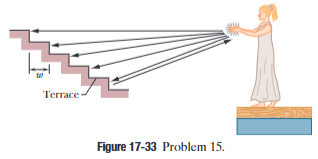
\includegraphics[width=0.33\textwidth]{17-33.png} 
            % \label{fig:wrapfig}
        \end{wrapfigure}
        A handclap on stage in an amphitheater sends out sound waves that scatter from terraces of width $w = 0.75$ m (Fig. 17-33). 
        The sound returns to the stage as a periodic series of pulses, one from each terrace; the parade of pulses sounds like a played note. 
        (a) Assuming that all the rays in Fig. 17-33 are horizontal, find the frequency at which the pulses return (that is, the frequency of the perceived note). 
        (b) If the width $w$ of the terraces were smaller, would the frequency be higher or lower?

        \subsection{Solution (a)}
            With each step, the sound would have to travel an additional distance of $2w$.
            If we divide the speed of all these sounds by the extra distance to travel, we would get the frequency of the return of the pulse rays.
            \begin{equation}
                f   =   \frac{v}{\Delta x}
                    =   \frac{343\,\unit{\meter/\second}}{2(0.75\,\unit{\meter})}
                    =   \boxed{228.67\,\unit{\hertz}}
            \end{equation}
        
        \subsection{Solution (b)}
            The frequency would be higher.

    \pagebreak
    \section{Problem 17}
        Two loudspeakers are located 3.35 m apart on an outdoor stage. 
        A listener is 18.3 m from one and 19.5 m from the other. 
        During the sound check, a signal generator drives the two speakers in phase with the same amplitude and frequency.
        The transmitted frequency is swept through the audible range (20 Hz to 20 kHz). 
        (a) What is the lowest frequency $f_{\rm min,1}$ that gives minimum signal (destructive interference) at the listener's location? 
        By what number must $f_{\rm min,1}$ be multiplied to get (b) the second lowest frequency $f_{\rm min,2}$ that gives minimum signal and (c) the third lowest frequency $f_{\rm min,3}$ that gives minimum signal? 
        (d) What is the lowest frequency $f_{\rm max,1}$ that gives maximum signal (constructive interference) at the listener's location? 
        By what number must $f_{\rm max,1}$ be multiplied to get (e) the second lowest frequency $f_{\rm max,2}$ that gives maximum signal and (f) the third lowest frequency $f_{\rm max,3}$ that gives maximum signal?

        \subsection{Solution (a)}
            For there to be destructive interference, the path length difference ($19.5\unit{\meter} - 18.3\unit{\meter} = 1.2\unit{\meter}$) divided by the wavelength ($\lambda$) must be equal to a number $n$ which is 0.5 more or less than a natural number.
            For the shortest possible, we can start with $n = 0.5$.
            \begin{align}
                \lambda &=  \frac{1.2\,\unit{\meter}}{0.5}
                    =   2.4\,\unit{\meter}
            \end{align}

            From here, we can calculate the frequency from $v = \lambda f$.
            The velocity is the speed of sound.
            \begin{align}
                f   &=  \frac{v}{\lambda}
                    =   \frac{343\,\unit{\meter/\second}}{2.4\,\unit{\meter}}
                    =   \boxed{142.9\,\unit{\hertz}}
            \end{align}

            This is the least. 
            You can check.
        
        \subsection{Solution (b)}
            Same thing, just for $n = 1.5$.
            \begin{align}
                f   &=  \frac{v}{\lambda}
                    =   \frac{v}{\Delta L/n}
                    =   \frac{nv}{\Delta L}
                    =   \frac{1.5 * 343\,\unit{\meter/\second}}{1.2\,\unit{\meter}}
                    =   \boxed{428.75\,\unit{\hertz}}
            \end{align}
        
        \subsection{Solution (c)}
            Same thing, just for $n = 2.5$.
            \begin{align}
                f   &=  \frac{v}{\lambda}
                    =   \frac{v}{\Delta L/n}
                    =   \frac{nv}{\Delta L}
                    =   \frac{2.5 * 343\,\unit{\meter/\second}}{1.2\,\unit{\meter}}
                    =   \boxed{714.58\,\unit{\hertz}}
            \end{align}

        \subsection{Solution (d)}
            Same thing as part (a), just for constructive interference, $n$ would be equal to a natural number or zero.
            $n$ being equal to zero would only be the case when there is $\Delta L$ is equal to zero or the wavelength is infinite.
            The former is not the case and the latter would result in a frequency that is out of the boundaries of the frequency values, so we can just start at $n = 1$.
            \begin{align}
                f   &=  \frac{v}{\lambda}
                    =   \frac{v}{\Delta L/n}
                    =   \frac{nv}{\Delta L}
                    =   \frac{1 * 343\,\unit{\meter/\second}}{1.2\,\unit{\meter}}
                    =   \boxed{285.83\,\unit{\hertz}}
            \end{align}
        
        \subsection{Solution (e)}
            Same thing, just for $n = 2$.
            \begin{align}
                f   &=  \frac{v}{\lambda}
                    =   \frac{v}{\Delta L/n}
                    =   \frac{nv}{\Delta L}
                    =   \frac{2 * 343\,\unit{\meter/\second}}{1.2\,\unit{\meter}}
                    =   \boxed{571.67\,\unit{\hertz}}
            \end{align}
        
        \subsection{Solution (f)}
            Same thing, just for $n = 3$.
            \begin{align}
                f   &=  \frac{v}{\lambda}
                    =   \frac{v}{\Delta L/n}
                    =   \frac{nv}{\Delta L}
                    =   \frac{3 * 343\,\unit{\meter/\second}}{1.2\,\unit{\meter}}
                    =   \boxed{857.5\,\unit{\hertz}}
            \end{align}

    \pagebreak
    \section{Problem 19}
        \begin{wrapfigure}{r}{0.33\textwidth}
            % \vspace{-30pt}
            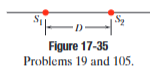
\includegraphics[width=0.33\textwidth]{17-35.png} 
            % \label{fig:wrapfig}
        \end{wrapfigure}
        Figure 17-35 shows two isotropic point sources of sound, $S_1$ and $S_2$. 
        The sources emit waves in phase at wavelength 0.50 m; they are separated by D = 1.75 m. 
        If we move a sound detector along a large circle centered at the midpoint between the sources, at how many points do waves arrive at the detector (a) exactly in phase and (b) exactly out of phase?

        \subsection{Solution (a)}
            We are looking for cases where the remainder of $\frac{\Delta L}{\lambda}$ and 1 is 0.5.
            \begin{equation}
                \frac{\Delta L}{\lambda} \equiv 0.5 \mod 1
            \end{equation}

            Suppose that the radius of the circle is $R$.
            This would create two vectors, once for the distance from $S_1$ and $S_2$.
            \begin{align}
                &\vec{L}_1  =   R\begin{pmatrix}
                    \cos(\theta) + \frac{D}{2}\\
                    \sin(\theta)
                \end{pmatrix}
                &\vec{L}_2  =   R\begin{pmatrix}
                    \cos(\theta) - \frac{D}{2}\\
                    \sin(\theta)
                \end{pmatrix}
            \end{align}

            From this, we can create a formula for $\Delta L$ and graph it on a plane.
            \begin{align}
                \left| \left| L_1 \right| \right|   &=  \sqrt{\left( \cos(\theta) + \frac{D}{2} \right)^2 + \sin^2(\theta)}\\
                \left| \left| L_2 \right| \right|   &=  \sqrt{\left( \cos(\theta) - \frac{D}{2} \right)^2 + \sin^2(\theta)}\\
                \Delta L    &=  \sqrt{\left( \cos(\theta) - \frac{D}{2} \right)^2 + \sin^2(\theta)} - \sqrt{\left( \cos(\theta) + \frac{D}{2} \right)^2 + \sin^2(\theta)}
            \end{align}
            \begin{center}
                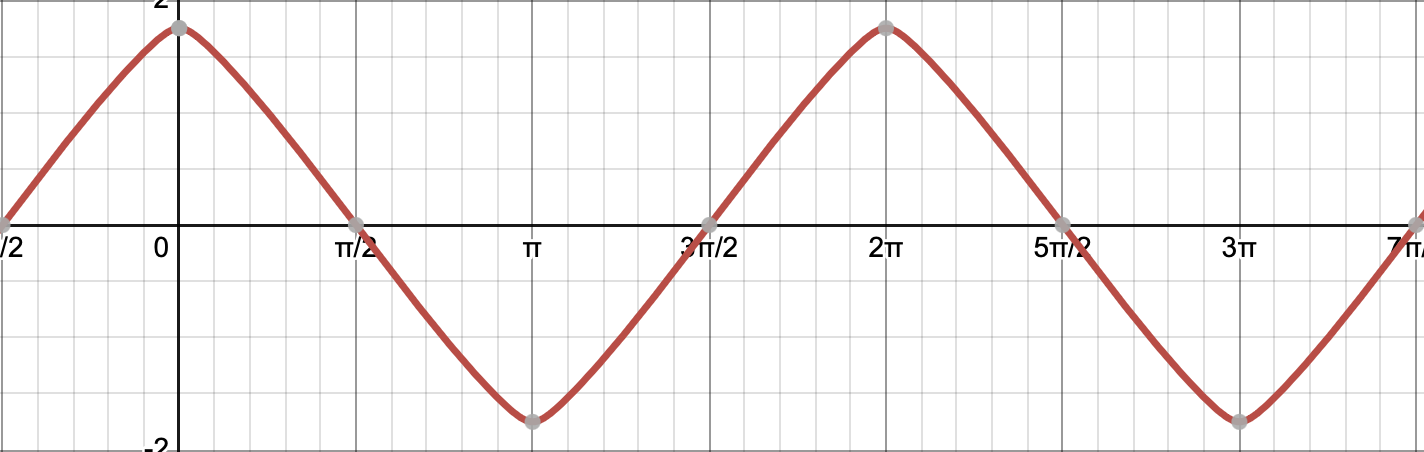
\includegraphics[width=\textwidth]{Fig-19-1.png}
            \end{center}

            Looking at it here, we can see that between 0 and $\frac{\pi}{2}$, it does not change direction once.
            Knowing this, we can first calculate the variation in the value of $\Delta L$.
            This applies for between when $\theta = 0$ and $\theta = \frac{\pi}{2}$.
            \begin{align}
                \Delta L(0) &=  \sqrt{\left( \cos(0) - \frac{D}{2} \right)^2 + \sin^2(0)} - \sqrt{\left( \cos(0) + \frac{D}{2} \right)^2 + \sin^2(0)}\\
                    &=  \sqrt{\left( \cos(0) - \frac{D}{2} \right)^2} - \sqrt{\left( \cos(0) + \frac{D}{2} \right)^2}
                    =   -D\\
                \Delta L\left( \frac{\pi}{2} \right)    &=  \sqrt{\left( \frac{D}{2} \right)^2 + \sin^2(0)} - \sqrt{\left( \frac{D}{2} \right)^2 + \sin^2(0)}
                    =   0
            \end{align}

            In any case, we would only have to find the points at which $\frac{\Delta L}{\lambda} \equiv 0.5 \mod 1$ for $0 \leq \Delta L \leq D$.
            Since $\lambda = 0.5$, dividing everything by $\lambda$ would be equivalent to multiplying by 2, so we can use that for the limits.
            \begin{gather}
                0 \leq \Delta L \leq D\\
                0 \leq \frac{\Delta L}{\lambda} \leq 2D\\
                0 \leq \frac{L}{\lambda} \leq 3.5
            \end{gather}

            At this point, we could just count the cases that work for the requirements.
            If one of the boundary cases applies, we should only consider it as half of a case that works.\\
            1: $0 \leq 0.5 \leq 3.5$;
            2: $0 \leq 1.5 \leq 3.5$;
            3: $0 \leq 2.5 \leq 3.5$;
            3.5: $0 \leq 3.5 \leq 3.5$\\
            This leaves us with three and a half cases of congruence in the first quarter of the circle.
            Multiplying it by the four quarters of the circle, we get a total of $3.5 * 4 = \boxed{14}$ in-phase spots.

        \subsection{Solution}
            Soem thing, just for $\frac{\Delta L}{\lambda} \equiv 0 \mod 1$.\\
            0.5: $0 \leq 0 \leq 3.5$;
            1.5: $0 \leq 1 \leq 3.5$;
            2.5: $0 \leq 2 \leq 3.5$;
            3.5: $0 \leq 3 \leq 3.5$\\
            This leaves us with three and a half cases of congruence in the first quarter of the circle.
            Multiplying it by the four quarters of the circle, we get a total of $3.5 * 4 = \boxed{14}$ in-phase spots.

    \pagebreak
    \section{Problem 20}
        \begin{center}
            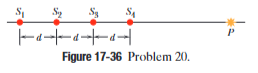
\includegraphics[width=0.5\textwidth]{17-36.png} 
        \end{center}
        Figure 17-36 shows four isotropic point sources of sound that are uniformly spaced on an x axis. 
        The sources emit sound at the same wavelength $\lambda$ and same amplitude $s_m$, and they emit in phase. 
        A point P is shown on the x axis. 
        Assume that as the sound waves travel to P, the decrease in their amplitude is negligible. 
        What multiple of $s_m$ is the amplitude of the net wave at P if distance d in the figure is (a) $\lambda$/4, (b) $\lambda$/2, and (c) $\lambda$?

        \subsection{Solution (a)}
            We can pair off these points and calculate the total wave from each.
            First do $S_1$ and $S_2$, then $S_3$ and $S_4$.
            \begin{align}
                \phi    &=  \frac{\Delta L}{\lambda}\,2\pi\\
                \phi_1  &=  \frac{\lambda/4}{\lambda}\,2\pi
                    =   \frac{\pi}{2}\\
                \phi_2  &=  \frac{\lambda/4}{\lambda}\,2\pi
                    =   \frac{\pi}{2}
            \end{align}

            These would initially intersect at $S_2$ and $S_4$ respectively, which are a distance of $2 * \frac{\lambda}{4} = \frac{\lambda}{2}$ apart.
            The two previously resultant waves would be identical.
            We can from here find the result of the interference of the resultant waves.
            \begin{align}
                \phi_3  &=  \frac{\lambda/2}{\lambda}\,2\pi
                    =   \pi
            \end{align}

            This results in completely destructive interference.
            As a result of this the multiple now would be \boxed{0}.

        \subsection{Solution (b)}
            This time, just do $S_1$ and $S_2$, then $S_3$ and $S_4$.
            \begin{align}
                \phi    &=  \frac{\Delta L}{\lambda}\,2\pi\\
                \phi_1  &=  \frac{\lambda/2}{\lambda}\,2\pi
                    =   \pi\\
                \phi_2  &=  \frac{\lambda/2}{\lambda}\,2\pi
                    =   \pi
            \end{align}

            Both of these have destructive interference, so in total the multiple of it would be \boxed{0}.

        \subsection{Solution (c)}
            Lastly, first do $S_1$ and $S_2$ as well as $S_3$ and $S_4$.
            \begin{align}
                \phi    &=  \frac{\Delta L}{\lambda}\,2\pi\\
                \phi_1  &=  \frac{\lambda}{\lambda}\,2\pi
                    =   2\pi\\
                \phi_2  &=  \frac{\lambda}{\lambda}\,2\pi
                    =   2\pi
            \end{align}

            Both of these are construvtive interference, so it doubles the first.
            We can combine the two we presently have, which ar $2\lambda$ apart.
            \begin{align}
                \phi_3  &=  \frac{2\lambda}{\lambda}\,2\pi
                    =   4\pi
            \end{align}

            This also qualfies as constructive intereference, so the net multipland would be \boxed{4}.

    \pagebreak
    \section{Problem 25}
        A sound wave of frequency 300 Hz has an intensity of 1.00 \unit{\micro\watt/\meter^2}. 
        What is the amplitude of the air oscillations caused by this wave?

        \subsection{Solution}
            There is an equation that relates amplitude to intensity.
            \begin{equation}
                I   =   \frac{1}{2}\rho v \omega^2 s_m^2
            \end{equation}

            We can solve for the amplitude ($s_m$).
            \begin{gather}
                s_m^2   =   \frac{2I}{\rho v \omega^2}\\
                s_m =   \sqrt{\frac{2I}{\rho v \omega^2}}
            \end{gather}

            We have the density of air ($\rho$), speed of sound ($v$), intensity ($I$), and frequency ($f$).
            The latter can be easily converted into angular speed ($\omega$).
            \begin{gather}
                \omega  =   2\pi f\\
                \begin{align}
                    s_m &=  \sqrt{\frac{2I}{\rho v (2\pi f)^2}}
                        =   \sqrt{\frac{2(1.00\,\unit{\micro\watt/\meter^2})}{1.21\,\unit{\kilo\gram/\meter^3} * 343\,\unit{\meter/\second} * (2\pi\,300\,\unit{\hertz})^2}}\\
                        &=  \boxed{3.68\E{-8}\,\unit{\meter}}
                \end{align}
            \end{gather}

    \pagebreak
    \section{Problem 27}
        A certain sound source is increased in sound level by 30.0 dB. By what multiple is (a) its intensity increased and (b) its pressure amplitude increased?

        \subsection{Solution (a)}
            Sound level is described by an equation.
            \begin{equation}
                \beta = (10\,\unit{\deci\bel}) \log_{10} \frac{I}{I_0}
            \end{equation}

            We can turn this into a change formula (involving $\Delta$) and solve from there.
            \begin{gather}
                \begin{align}
                    \Delta \beta    &=  \beta_f - \beta_i
                        =   (10\,\unit{\deci\bel}) \log_{10} \frac{I_f}{I_0} - (10\,\unit{\deci\bel}) \log_{10} \frac{I_i}{I_0}\\
                        &=  (10\,\unit{\deci\bel}) \left( \log_{10} \frac{I_f}{I_0} - \log_{10} \frac{I_i}{I_0} \right)\\
                        &=  (10\,\unit{\deci\bel}) \log_{10} \frac{I_f}{I_i}
                        =   30.0\,\unit{\deci\bel}
                \end{align}\\
                \log_{10} \frac{I_f}{I_i} = 3\\
                \frac{I_f}{I_i} = \boxed{10^3}
            \end{gather}

        \subsection{Solution (b)}
            Intensity has an equation we know. So does pressure amplitude.
            \begin{gather}
                I   =   \frac{1}{2}\rho v \omega^2 s_m^2\\
                \Delta p_m  =   (v\rho\omega)s_m
            \end{gather}

            In this case, the only thing that changes in either equation is the value of $s_m$.
            If we can find the change multiplicand of $s_m$, we can find the change multiplicand of $\Delta p_m$.
            \begin{gather}
                \frac{I_f}{I_i} = \frac{\frac{1}{2}\rho v \omega^2 s_{m,f}^2}{\frac{1}{2}\rho v \omega^2 s_{m,i}^2}
                    =   \frac{s_{m,f}^2}{s_{m,i}^2}
                    =   10^3\\
                \frac{s_{m,f}}{s_{m,i}} =   \sqrt{10^3}
                    =   \boxed{31.62}
            \end{gather}

    \pagebreak
    \section{Problem 29}
        A point source emits sound waves isotropically. 
        The intensity of the waves 2.50 m from the source is $1.91\E{-4}\,\unit{\watt/\meter^2}$. 
        Assuming that the energy of the waves is conserved, find the power of the source.

        \subsection{Solution}
            The formula for power from intensity is related directly to the area covered.
            \begin{equation}
                P   =   IA
            \end{equation}

            In this case, isotropic emission would result in the waves exiting in a spherical manner.
            The equation for the surface area of a sphere is $4\pi r^2$.
            We can use these equations to find the power.
            \begin{align}
                P   &=  IA
                    =   1.91\E{-4}\,\unit{\watt/\meter^2} \times 4\pi (2.5\,\unit{\meter})^2
                    =   \boxed{0.0150\,\unit{\watt}}
            \end{align}

    \pagebreak
    \section{Problem 35}
        A point source emits 30.0 W of sound isotropically. 
        A small microphone intercepts the sound in an area of 0.750 \unit{\centi\meter^2}, 200 m from the source. 
        Calculate (a) the sound intensity there and (b) the power intercepted by the microphone.

        \subsection{Solution}

    \pagebreak
    \section{Problem 39}
        (a) Find the speed of waves on a violin string of mass 800 mg and length 22.0 cm if the fundamental frequency is 920 Hz. 
        (b) What is the tension in the string? 
        For the fundamental, what is the wavelength of (c) the waves on the string and (d) the sound waves emitted by the string?


        \subsection{Solution}

    \pagebreak
    \section{Problem 41}
        A violin string 15.0 cm long and fixed at both ends oscillates in its n = 1 mode. 
        The speed of waves on the string is 250 m/s, and the speed of sound in air is 348 m/s. 
        What are the (a) frequency and (b) wavelength of the emitted sound wave?

        \subsection{Solution}

    \pagebreak
    \section{Problem 47}
        A well with vertical sides and water at the bottom resonates at 7.00 Hz and at no lower frequency. 
        The air-filled portion of the well acts as a tube with one closed end (at the bottom) and one open end (at the top). 
        The air in the well has a density of 1.10 kg/m 3 and a bulk modulus of $1.33\E{5}\,\unit{\pascal}$. 
        How far down in the well is the water surface?

        \subsection{Solution}

    \pagebreak
    \section{Problem 49}
        A violin string 30.0 cm long with linear density 0.650 g/m is placed near a loudspeaker that is fed by an audio oscillator of variable frequency. 
        It is found that the string is set into oscillation only at the frequencies 880 and 1320 Hz as the frequency of the oscillator is varied over the range 500 to 1500 Hz.
        What is the tension in the string?

        \subsection{Solution}

    \pagebreak
    \section{Problem 51}
        The A string of a violin is a little too tightly stretched. 
        Beats at 4.00 per second are heard when the string is sounded together with a tuning fork that is oscillating accurately at concert A (440 Hz).
        What is the period of the violin string oscillation?

        \subsection{Solution}

    \pagebreak
    \section{Problem 53}
        Two identical piano wires have a fundamental frequency of 600 Hz when kept under the same tension. 
        What fractional increase in the tension of one wire will lead to the occurrence of 6.0 beats/s when both wires oscillate simultaneously?

        \subsection{Solution}

    \pagebreak
    \section{Problem 55}
        A whistle of frequency 540 Hz moves in a circle of radius 60.0 cm at an angular speed of 15.0 rad/s. 
        What are the (a) lowest and (b) highest frequencies heard by a listener a long distance away, at rest with respect to the center of the circle?

        \subsection{Solution}

    \pagebreak
    \section{Problem 57}
        A state trooper chases a speeder along a straight road; both vehicles move at 160 km/h. 
        The siren on the trooper's vehicle produces sound at a frequency of 500 Hz. 
        What is the Doppler shift in the frequency heard by the speeder?

        \subsection{Solution}

    \pagebreak
    \section{Problem 61}
        A bat is flitting about in a cave, navigating via ultrasonic bleeps. 
        Assume that the sound emission frequency of the bat is 39 000 Hz. 
        During one fast swoop directly toward a flat wall surface, the bat is moving at 0.025 times the speed of sound in air. 
        What frequency does the bat hear reflected off the wall?

        \subsection{Solution}

    \pagebreak
    \section{Problem 63}
        An acoustic burglar alarm consists of a source emitting waves of frequency 28.0 kHz. 
        What is the beat frequency between the source waves and the waves reflected from an intruder walking at an average speed of 0.950 m/s directly away from the alarm?

        \subsection{Solution}

    \pagebreak
    \section{Problem 71}

        \subsection{Solution}

    \pagebreak
    \section{Problem 81}

        \subsection{Solution}

    \pagebreak
    \section{Problem 87}

        \subsection{Solution}

    \pagebreak
    \section{Problem 99}

        \subsection{Solution}

    \pagebreak
    \section{Problem 107}

        \subsection{Solution}

    \pagebreak

    \tableofcontents
\end{document}